\documentclass[12pt,a4paper]{article}
\usepackage{amsmath}
\usepackage{amsfonts}
\usepackage{amssymb}
\usepackage{graphicx}
\usepackage{secdot}
\usepackage{amsmath}
\usepackage{commath}
\usepackage[left=2cm,right=2cm,top=2cm,bottom=2cm]{geometry}

\author{Shibayan Biswas, AE21B109\\ Department of Aerospace Engineering\\ IIT Madras}
\title{Assignment - 8}
\date{October 28, 2022}
\begin{document}
\maketitle
\hline
\section{Identify the Frequencies:}
Given a time signal, $g$(t), the Forward Fourier transform can help evaluate the signal in the frequency domain, $\hat{g}$(f). The transformation is given by:
\begin{equation}
    \text{$\hat{g}$}(f) = \text{$\int_{-\infty}^{\infty}{\text{g}(t) \text{exp}(-2 \pi ift) \text{dt}}$}
\end{equation}
In this part of the assignment we have to use the information and the time signal given in the file "signal.inp". Based on this certain tasks are given to be performed. Before moving ahead let us have a brief introduction to Fourier transform.
\subsection{Fourier transform:}
A Fourier transform is a mathematical transform that decomposes functions into frequency components, which are represented by the output of the transform as a function of frequency. Most commonly functions of time or space are transformed, which will output a function depending on temporal frequency or spatial frequency respectively. That process is also called analysis. An example application would be decomposing the waveform of a musical chord into terms of the intensity of its constituent pitches. The term Fourier transform refers to both the frequency domain representation and the mathematical operation that associates the frequency domain representation to a function of space or time.\\
\\The Fourier transform of a function is a complex-valued function representing the complex sinusoids that comprise the original function. For each frequency, the magnitude (absolute value) of the complex value represents the amplitude of a constituent complex sinusoid with that frequency, and the argument of the complex value represents that complex sinusoid's phase offset. If a frequency is not present, the transform has a value of 0 for that frequency. The Fourier transform is not limited to functions of time, but the domain of the original function is commonly referred to as the time domain. The Fourier inversion theorem provides a synthesis process that recreates the original function from its frequency domain representation.\\
\clearpage
\noindent
Functions that are localized in the time domain have Fourier transforms that are spread out across the frequency domain and vice versa, a phenomenon known as the uncertainty principle. The critical case for this principle is the Gaussian function, of substantial importance in probability theory and statistics as well as in the study of physical phenomena exhibiting normal distribution (e.g., diffusion). The Fourier transform of a Gaussian function is another Gaussian function. Joseph Fourier introduced the transform in his study of heat transfer, where Gaussian functions appear as solutions of the heat equation.\\
\\The Fourier transform can be formally defined as an improper Riemann integral, making it an integral transform, although this definition is not suitable for many applications requiring a more sophisticated integration theory. For example, many relatively simple applications use the Dirac delta function, which can be treated formally as if it were a function, but the justification requires a mathematically more sophisticated viewpoint.\\
\subsection{Plot of the Amplitude of each Frequency:}
In this particular section, I have provided the plot of the Amplitude of each Frequency for the time signal given in the file "signal.inp". The figure for the given plot is shown below:
\begin{figure}[!ht]
	\begin{center}
		\framebox{
			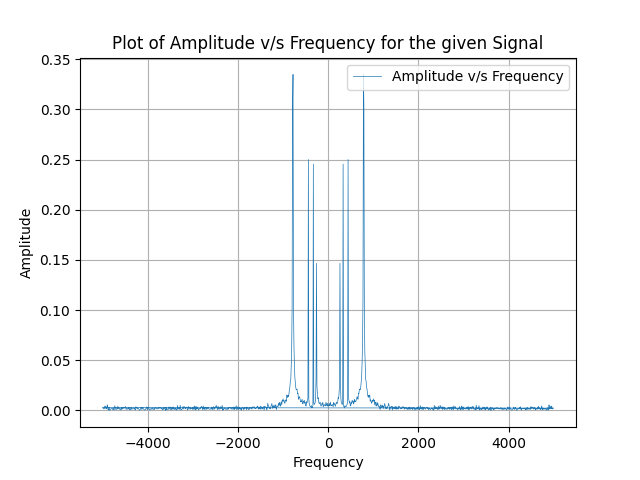
\includegraphics[scale=1.0]{Figure_1.png}
		}
	\end{center}
	\caption{Plot of the Amplitude of each Frequency}
\end{figure}
\clearpage
\noindent
In the second program file that is attached to this folder, I have calculated the magnitudes of the different frequencies for the time signal given in the file "signal.inp".
\subsection{Nyquist’s Sampling Theorem:}
The Nyquist Sampling Theorem states that a band limited continuous-time signal can be sampled and perfectly reconstructed from its samples if the waveform is sampled over twice as fast as it's highest frequency component. \\
\\Nyquist limit is the highest frequency component that can be accurately represented as:
\begin{equation}
    \text{$f_{c}$} < \frac{\text{$f_s$}}{2}
\end{equation}
The sampling frequency should be at least twice the highest frequency contained in the signal which can be accurately represented as:
\begin{equation}
    \text{$f_{s}$} \geq \text{$2f_c$}
\end{equation}
The Nyquist–Shannon sampling theorem is a theorem in the field of signal processing which serves as a fundamental bridge between continuous-time signals and discrete-time signals. It establishes a sufficient condition for a sample rate that permits a discrete sequence of samples to capture all the information from a continuous-time signal of finite bandwidth.\\
\\Strictly speaking, the theorem only applies to a class of mathematical functions having a Fourier transform that is zero outside of a finite region of frequencies. Intuitively we expect that when one reduces a continuous function to a discrete sequence and interpolates back to a continuous function, the fidelity of the result depends on the density (or sample rate) of the original samples. The sampling theorem introduces the concept of a sample rate that is sufficient for perfect fidelity for the class of functions that are band-limited to a given bandwidth, such that no actual information is lost in the sampling process. It expresses the sufficient sample rate in terms of the bandwidth for the class of functions. The theorem also leads to a formula for perfectly reconstructing the original continuous-time function from the samples.\\
\\Perfect reconstruction may still be possible when the sample-rate criterion is not satisfied, provided other constraints on the signal are known . In some cases (when the sample-rate criterion is not satisfied), utilizing additional constraints allows for approximate reconstructions.
\subsection{Notes (or Chords) represented by the given Signal:}
I have calculated magnitudes of the different frequencies for the time signal given in the file ”signal.inp" in the second program file that is attached to this folder. Over there the values of the values of the frequencies obtained were 330.0, 440.0, 780.0 and 790.0. The note (or chord) corresponding to frequency 330.0 is "E", the note (or chord) corresponding to frequency 440.0 is "A" and the note (or chord) corresponding to frequency range between 780.0 and 790.0 is "G" respectively. The following result has been obtained from the Chart of Frequency vs Note (or Chord).
\clearpage
\section{Remove the Noise:}
In this part of the assignment we have to use the information and the time signal given in the file "noise.inp". This signal has “broadband noise”, i.e. noise that may exist in a large frequency range. However, in the present scenario, we see that the noise is of a small amplitude (always less than
0.01). Based on this certain tasks are given to be performed.
\subsection{Plot of the Amplitude of each Frequency:}
In this particular section, I have provided the plot of the Amplitude of each Frequency for the time signal given in the file "noise.inp". The figure for the given plot is shown below:\\
\begin{figure}[!ht]
	\begin{center}
		\framebox{
			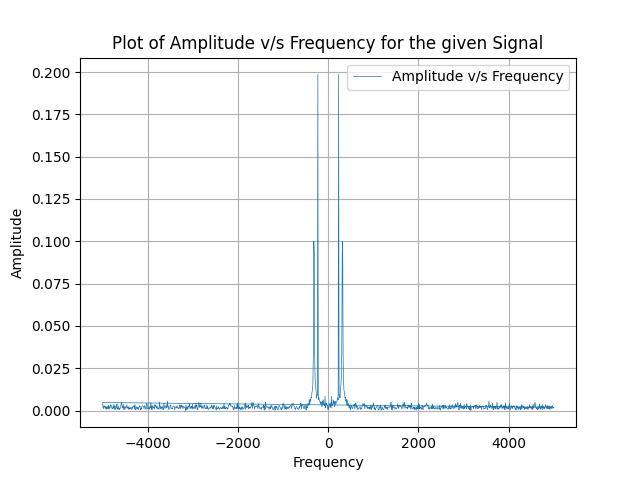
\includegraphics[scale=1.0]{Figure_2.png}
		}
	\end{center}
	\caption{Plot of the Amplitude of each Frequency}
\end{figure}
\noindent
\\In the fourth program file that is attached to this folder, I have calculated the magnitudes of the true frequencies for the time signal given in the file "noise.inp".
\subsection{Plot of Signal v/s Time (Original and Modified):}
In this section I have provided the plot of Signal v/s Time for the time signal given in the file "noise.inp" containing the original plot and the plot after eliminating the true frequencies from the frequency domain. The figure for the given plot and the figure of the given plot magnified with respect to Time $\epsilon$ [0.04, 0.06] is shown below:
\begin{figure}[!ht]
	\begin{center}
		\framebox{
			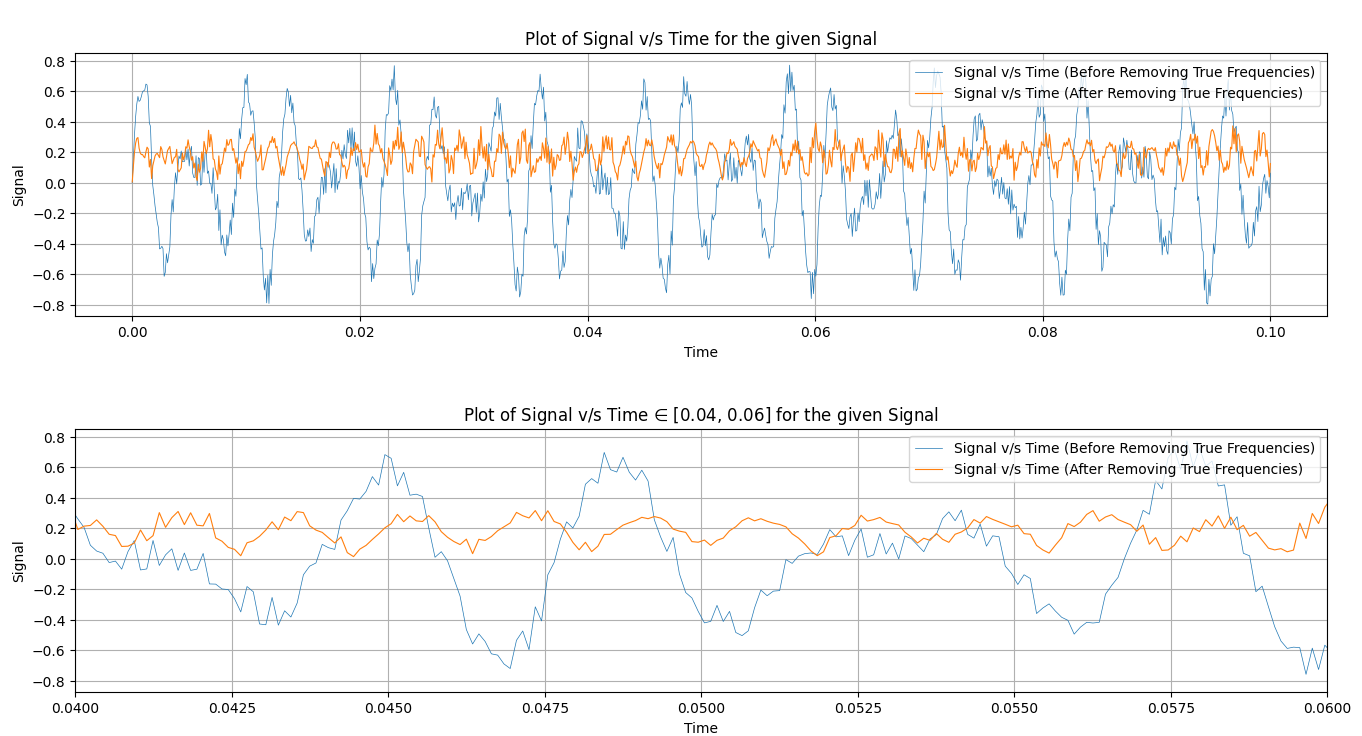
\includegraphics[scale=0.45]{Figure_3.png}
		}
	\end{center}
	\caption{Plot of Signal v/s Time (Original and Modified)}
\end{figure}
\subsection{Plot of FFT of the Five Point Median Average time signal:}
In this section I have provided the plot of FFT of the Five Point Median Average time signal for the time signal given in the file "noise.inp". The figure for the given plot is shown below:
\begin{figure}[!ht]
	\begin{center}
		\framebox{
			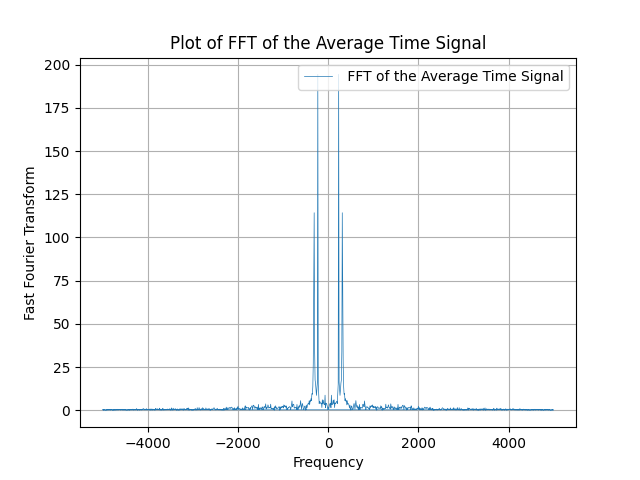
\includegraphics[scale=0.8]{Figure_4.png}
		}
	\end{center}
	\caption{Plot of FFT of the Five Point Median Average time signal}
\end{figure}
\clearpage
\noindent
From the above plot of FFT of the Five Point Median Average time signal for the time signal given in the file "noise.inp", I conclude that most of the noise from the original time signal given in the file "noise.inp" has been removed. The peaks present in the above plot are same as the plot of the Amplitude of each Frequency for the time signal given in the file "noise.inp". The only change that has taken place is that the plot has smoothed.
\end{document}
